%==============================================================================
% Praca dyplomowa (WSIiZ) — plik główny
%==============================================================================

\documentclass[pl,auxsup]{wsiz}

%------------------------------------------------------------------------------
% JĘZYK / KODOWANIE (pdfLaTeX)
%------------------------------------------------------------------------------
\usepackage[main=polish]{babel}
\addto\captionspolish{%
  \renewcommand{\contentsname}{Spis treści}%
  \renewcommand{\listfigurename}{Spis rysunków}%
  \renewcommand{\listtablename}{Spis tabel}%
  \renewcommand{\figurename}{Rys.}%
  \renewcommand{\tablename}{Tab.}%
}


%------------------------------------------------------------------------------
% MATEMATYKA (włącz, jeśli realnie używasz)
%------------------------------------------------------------------------------
\usepackage{mathtools}
\usepackage{amssymb}

%------------------------------------------------------------------------------
% FLOATY (tylko jeśli używasz [H])
%------------------------------------------------------------------------------
\usepackage{float}
\usepackage{subcaption}
\usepackage{xurl} % lepsze łamanie długich adresów
\usepackage{tikz}
\usetikzlibrary{positioning,fit,shapes.geometric,arrows.meta}

%------------------------------------------------------------------------------
% TABELE (włączaj wg potrzeby)
%------------------------------------------------------------------------------
\usepackage{booktabs}
\usepackage{multirow}
\usepackage{tabularx}
\usepackage{array}
\usepackage{makecell}
\usepackage[flushleft]{threeparttable}

% Kolumna X-centrowana o kontrolowanej szerokości
\newcolumntype{C}[1]{>{\hsize=#1\hsize\centering\arraybackslash}X}

%------------------------------------------------------------------------------
% LISTINGI (kod źródłowy)
%------------------------------------------------------------------------------
\usepackage{listings}
\usepackage{listingsutf8}
\usepackage{xcolor}

% Nazwy po polsku (listings)
\renewcommand{\lstlistlistingname}{Spis listingów}
\renewcommand{\lstlistingname}{Listing}



% Kolory dla kodu (bez konfliktu z "green")
\definecolor{codegreen}{rgb}{0,0.6,0}
\definecolor{codegray}{rgb}{0.5,0.5,0.5}

% Ustawienia listings — jeden spójny blok
\lstdefinestyle{mystyle}{
  inputencoding=utf8,
  extendedchars=true,
  basicstyle=\ttfamily\footnotesize,
  breaklines=true,
  numbers=left,
  numberstyle=\tiny\color{codegray},
  numbersep=6pt,
  showstringspaces=false,
  tabsize=2,
  keywordstyle=\color{blue},
  commentstyle=\color{codegreen},
  stringstyle=\color{red}, 
}
\lstset{style=mystyle}

%------------------------------------------------------------------------------
% PODKREŚLANIE (ulem) + NUMERY LINII (lineno)
%------------------------------------------------------------------------------
\usepackage[normalem]{ulem}
\usepackage{lineno}

%------------------------------------------------------------------------------
% CYTOWANIA (przydatne z babel)
%------------------------------------------------------------------------------
\usepackage{csquotes}

%------------------------------------------------------------------------------
% ZMIENNE DOKUMENTU (dla klasy wsiz)
%------------------------------------------------------------------------------
\author{Piotr Ostrowski}
\shortauthor{P. Ostrowski}
\noAlbum{69826}

\titlePL{Projekt systemu OSK-Manager do zarządzania ośrodkiem szkolenia kierowców}
\titleEN{Design of the OSK-Manager System for Driving School Management}

\shorttitlePL{Projekt systemu OSK-Manager}
\shorttitleEN{Design of the OSK-Manager System}

\thesistype{}

\supervisor{}
% \secondsupervisor{dr Jan Nowak 2}

\degreeprogramme{INFORMATYKA}
\specialization{Technologie internetowe i mobilne}

\faculty{Kolegium Informatyki Stosowanej}

\acknowledgements{Serdecznie dziękuję \dots tu ciąg dalszych podziękowań np. dla promotora, żony, mężą, sąsiada/ki, psa, kota itp.}

\date{2026}

%------------------------------------------------------------------------------
% USTAWIENIA SPISU TREŚCI / NUMERACJI
%------------------------------------------------------------------------------
\setcounter{secnumdepth}{4}
\setcounter{tocdepth}{2}

\brokenpenalty=10000\relax

%==============================================================================
\begin{document}
%==============================================================================

%------------------------------------------------------------------------------
% Strona tytułowa + podziękowania
%------------------------------------------------------------------------------

\titlepages
% Jeśli chcesz stopkę z autorem i skróconym tytułem (lewy dół) + numer w środku:
% \thesisheaders
\tableofcontents





%------------------------------------------------------------------------------
% Numeracja linii (włącz gdy potrzebujesz, np. do recenzji)
%------------------------------------------------------------------------------
\clearpage
% \linenumbers

%------------------------------------------------------------------------------
% Rozdziały
%-----------------------------------------------------------------------------

\selectlanguage{polish}
\chapter{Analiza problemu i przegląd istniejących rozwiązań}
\label{cha:analizaProblemu}

Niniejszy rozdział przedstawia problem, który rozwiązuje projektowany system OSK-Manager, oraz omawia wybrane istniejące rozwiązania przeznaczone dla ośrodków szkolenia kierowców. Analiza stanowi podstawę do określenia wymagań funkcjonalnych i niefunkcjonalnych systemu.

\section{Charakterystyka problemu}
\label{sec:charakterystykaProblemu}

Ośrodek szkolenia kierowców prowadzi równolegle wiele procesów organizacyjnych. Musi obsługiwać kursantów, instruktorów, pojazdy, kursy, lekcje teoretyczne i praktyczne, dostępność instruktorów, płatności, dokumentację oraz harmonogram jazd. Każdy z tych obszarów jest ze sobą powiązany. Przykładowo zaplanowanie jazdy praktycznej wymaga jednoczesnego sprawdzenia kursu kursanta, dostępności instruktora, dostępności pojazdu, rodzaju zajęć i przynależności wszystkich elementów do tej samej szkoły.

W praktyce wiele szkół jazdy korzysta z rozproszonych narzędzi: arkuszy kalkulacyjnych, papierowych kart, komunikatorów, zwykłego kalendarza oraz ręcznych notatek. Takie podejście jest wystarczające przy małej liczbie kursantów, ale wraz ze wzrostem liczby instruktorów, pojazdów i kursów zwiększa ryzyko błędów. Najpoważniejsze problemy to podwójne rezerwacje instruktora lub pojazdu, brak aktualnej informacji o dostępności, trudność w monitorowaniu postępów kursanta oraz brak jednego miejsca, w którym manager widzi stan szkoły.

Projekt OSK-Manager dotyczy systemu webowego wspierającego zarządzanie szkołą jazdy. Z analizy projektu wynika, że system obejmuje role użytkowników, ośrodki szkolenia kierowców, kursantów, instruktorów, pojazdy, kursy, lekcje, wydarzenia instruktorskie, dostępność, harmonogram, płatności i oceny. System ma zatem porządkować codzienną pracę OSK oraz wymuszać najważniejsze reguły biznesowe, takie jak brak kolizji terminów, spójność szkoły oraz przypisanie lekcji do konkretnego kursu.

\section{Skutki braku centralnego systemu}
\label{sec:skutkiBrakuSystemu}

Brak jednego systemu zarządzania powoduje problemy operacyjne i jakościowe. Manager może mieć trudność z szybkim ustaleniem, który instruktor jest dostępny, który pojazd może zostać użyty do jazdy oraz ilu kursantów znajduje się na konkretnym etapie szkolenia. Instruktor może nie mieć aktualnego widoku swoich zajęć, a kursant może nie wiedzieć, ile lekcji już odbył i jakie zajęcia są przed nim.

Szczególnie istotny jest problem planowania jazd praktycznych. Lekcja praktyczna wymaga jednoczesnej dostępności instruktora i pojazdu. Jeżeli harmonogram prowadzony jest ręcznie, łatwo doprowadzić do konfliktu terminów lub zaplanowania lekcji poza godzinami pracy instruktora. Dodatkowo pojazdy wymagają monitorowania statusu, terminów przeglądów, ubezpieczenia i dostępności.

Drugim problemem jest kontrola poprawności danych. Kursant może uczestniczyć w wielu kursach, ale każda lekcja musi należeć do konkretnego kursu. Instruktor i pojazd powinni być powiązani z tą samą szkołą, której dotyczy kurs. Takie reguły trudno egzekwować w arkuszu kalkulacyjnym, natomiast system informatyczny może sprawdzać je automatycznie.

\section{Cel projektowanego systemu}
\label{sec:celProjektowanegoSystemu}

Celem OSK-Manager jest dostarczenie aplikacji wspierającej codzienne zarządzanie ośrodkiem szkolenia kierowców. System powinien umożliwiać prowadzenie bazy kursantów, instruktorów, pojazdów i kursów, a także planowanie zajęć w sposób ograniczający ryzyko konfliktów.

System powinien wspierać trzy główne grupy użytkowników. Manager szkoły powinien zarządzać ośrodkami, personelem, kursami, pojazdami i harmonogramem. Instruktor powinien mieć dostęp do swoich zajęć oraz dostępności. Kursant powinien widzieć swoje kursy i lekcje. Dodatkowo administrator powinien mieć możliwość nadzoru nad danymi systemowymi i konfiguracją.

\section{Przegląd istniejących rozwiązań}
\label{sec:przegladRozwiazan}

Na rynku dostępne są systemy przeznaczone dla ośrodków szkolenia kierowców. Do porównania wybrano rozwiązania, które pokazują typowe funkcje oczekiwane w tej domenie: zarządzanie kursantami, instruktorami, pojazdami, harmonogramem, płatnościami i dokumentacją.

\subsection{CarDriveManager}
\label{subsec:carDriveManager}

CarDriveManager jest systemem CRM i kalendarzem dla szkół jazdy. Według materiałów producenta umożliwia zarządzanie grafikiem jazd, kursantami i płatnościami, a także obsługę bloków lekcyjnych oraz rozliczeń online\footnote{\url{https://cardrivemanager.com/start/}}. Rozwiązanie akcentuje automatyzację pracy biura oraz dostęp do informacji o kursantach i płatnościach w jednym miejscu.

Mocną stroną tego typu systemu jest kompleksowość. Obejmuje on wiele obszarów działalności OSK, od harmonogramu po płatności. Z perspektywy projektu OSK-Manager istotne jest podobne połączenie modułów operacyjnych, lecz z naciskiem na przejrzysty model ról, relacje pomiędzy szkołami, instruktorami i kursantami oraz automatyczne sprawdzanie reguł domenowych.

\subsection{Portal OSK}
\label{subsec:portalOsk}

Portal OSK to program do prowadzenia ośrodka szkolenia kierowców, który według opisu pozwala szybko wyszukiwać informacje o kursantach, pracownikach i pojazdach oraz wspiera prowadzenie OSK w sposób zgodny z wymaganiami organizacyjnymi\footnote{\url{https://www.portalosk.pl/}}. Rozwiązanie koncentruje się na centralizacji informacji potrzebnych w biurze szkoły jazdy.

Zaletą takiego systemu jest uporządkowanie danych administracyjnych. W porównaniu z OSK-Managerem można wskazać podobny cel: odejście od rozproszonych dokumentów i przeniesienie kluczowych danych do jednego systemu. OSK-Manager dodatkowo kładzie nacisk na dynamiczne wyliczanie dostępności instruktora na podstawie grafiku, wyjątków, blokad, urlopów i istniejących lekcji.

\subsection{OSKAdmin}
\label{subsec:oskAdmin}

OSKAdmin jest aplikacją do zarządzania szkołą jazdy. Producent wskazuje panel administracyjny dla biura i właściciela, obejmujący zarządzanie kursantami, instruktorami, pojazdami oraz kalendarzem zajęć\footnote{\url{https://oskadmin.pl/}}. System ma wspierać codzienne operacje szkoły i ograniczać ręczną pracę administracyjną.

OSKAdmin pokazuje, że kalendarz i zarządzanie personelem są kluczowymi elementami systemu dla OSK. W OSK-Managerze podobne wymaganie realizowane jest przez moduły harmonogramu, wydarzeń instruktorskich, dostępności oraz pojazdów. Ważne jest także rozróżnienie ról użytkowników, ponieważ inne operacje wykonuje manager, inne instruktor, a inne kursant.

\subsection{eOSK}
\label{subsec:eosk}

eOSK, oferowany przez Grupę IMAGE, opisuje moduły kursantów, instruktorów, pojazdów, finansów i zgłoszeń urzędowych\footnote{\url{https://www.grupaimage.eu/p696/eosk-program-do-zarzadzania-osk.html}}. Wśród funkcji wymieniane są między innymi zarządzanie szkoleniami, grafikami instruktorów, flotą pojazdów oraz przypomnieniami o terminach ważności przeglądów i ubezpieczeń.

To rozwiązanie pokazuje szeroki zakres potrzeb OSK. Dla OSK-Managera istotne są zwłaszcza moduły kursów, instruktorów i pojazdów. Projektowany system powinien zapewniać podstawę do dalszej rozbudowy o finanse, raportowanie i dokumentację, ale już na poziomie MVP musi poprawnie modelować relacje pomiędzy kursantem, kursem, lekcją, instruktorem i pojazdem.

\section{Porównanie rozwiązań}
\label{sec:porownanieRozwiazan}

\begin{table}[H]
  \centering
  \scriptsize
  \caption{Porównanie OSK-Manager z wybranymi rozwiązaniami}
  \label{tab:porownanieRozwiazanOsk}
  \begin{tabularx}{\textwidth}{>{\raggedright\arraybackslash}p{3cm}>{\raggedright\arraybackslash}X>{\raggedright\arraybackslash}X>{\raggedright\arraybackslash}X>{\raggedright\arraybackslash}X}
    \toprule
    \textbf{Kryterium} & \textbf{CarDrive Manager} & \textbf{Portal OSK} & \textbf{OSKAdmin / eOSK} & \textbf{OSK-Manager} \\
    \midrule
    Kursanci i kursy & Obsługa kursantów i postępów & Baza kursantów i informacji OSK & Moduły kursantów i szkoleń & Kursanci, kursy, typy kursów, status uczestnictwa i PKK \\
    \midrule
    Instruktorzy & Grafik instruktorów & Dane pracowników & Grafiki i dostępność instruktorów & Instruktorzy, kwalifikacje, przypisania do OSK i dostępność \\
    \midrule
    Pojazdy & Uwzględnienie pojazdów w grafiku & Informacje o pojazdach & Flota, przeglądy i ubezpieczenia & Pojazdy przypisane do OSK, status, zdjęcia i wykorzystanie w jazdach \\
    \midrule
    Harmonogram & Kalendarz jazd i bloków lekcyjnych & Organizacja pracy ośrodka & Kalendarz zajęć i grafiki & Harmonogram wyliczany z lekcji, wydarzeń i dostępności \\
    \midrule
    Reguły biznesowe & Automatyzacja procesów OSK & Centralizacja danych & Szeroki zakres modułów OSK & Spójność OSK, brak kolizji, lekcje tylko w ramach kursów \\
    \bottomrule
  \end{tabularx}
\end{table}

\section{Wnioski z analizy}
\label{sec:wnioskiAnaliza}

Analiza istniejących rozwiązań pokazuje, że systemy dla OSK skupiają się na kilku powtarzalnych obszarach: kursantach, instruktorach, pojazdach, harmonogramie, płatnościach i dokumentacji. Oznacza to, że projekt OSK-Manager odpowiada na realną potrzebę rynkową, a jego zakres jest zgodny z typowymi wymaganiami szkół jazdy.

Najważniejszym wyróżnikiem projektowanego systemu powinno być poprawne odwzorowanie reguł domenowych. System musi pilnować, aby lekcje należały do kursów, jazdy praktyczne miały przypisany pojazd, instruktorzy i pojazdy nie byli rezerwowani w tym samym czasie oraz aby dane dotyczyły właściwej szkoły. W kolejnych rozdziałach wymagania te zostaną rozwinięte w postaci wymagań funkcjonalnych, niefunkcjonalnych oraz modeli systemu.

\chapter{Opis biznesowy systemu}
\label{cha:opisBiznesowy}

OSK-Manager jest aplikacją webową służącą do zarządzania ośrodkiem szkolenia kierowców. System obejmuje obsługę szkół jazdy, użytkowników, kursantów, instruktorów, kursów, lekcji, pojazdów, dostępności, harmonogramu oraz wybranych danych rozliczeniowych. Poniżej przedstawiono wymagania funkcjonalne i niefunkcjonalne wynikające z zakresu projektu.

\section{Wymagania funkcjonalne}
\label{sec:wymaganiaFunkcjonalne}

Wymagania funkcjonalne określają funkcje, które powinien udostępniać system OSK-Manager.

\begin{enumerate}
  \item \textbf{WF-01. Logowanie użytkownika.} System powinien umożliwiać zalogowanie użytkownika za pomocą adresu e-mail i hasła.
  \item \textbf{WF-02. Obsługa sesji.} System powinien umożliwiać odświeżenie sesji, sprawdzenie aktualnego użytkownika oraz wylogowanie.
  \item \textbf{WF-03. Rejestracja użytkowników.} System powinien umożliwiać uprawnionym użytkownikom rejestrowanie kursantów i instruktorów.
  \item \textbf{WF-04. Role użytkowników.} System powinien rozróżniać role: kursant, instruktor, manager i administrator.
  \item \textbf{WF-05. Zarządzanie profilami.} System powinien umożliwiać edycję danych profilu użytkownika, w tym telefonu, opisu i avatara.
  \item \textbf{WF-06. Zarządzanie OSK.} System powinien umożliwiać managerowi tworzenie, edycję, listowanie i usuwanie własnych ośrodków szkolenia kierowców.
  \item \textbf{WF-07. Przypisanie użytkowników do OSK.} System powinien umożliwiać przypisywanie kursantów i instruktorów do wybranych szkół jazdy.
  \item \textbf{WF-08. Zarządzanie kursantami.} System powinien umożliwiać przeglądanie listy kursantów, szczegółów kursanta, notatek oraz numeru PKK.
  \item \textbf{WF-09. Zarządzanie instruktorami.} System powinien umożliwiać dodawanie, edycję, usuwanie i przeglądanie instruktorów przypisanych do OSK.
  \item \textbf{WF-10. Kwalifikacje instruktorów.} System powinien przechowywać informację, do jakich typów kursów uprawniony jest instruktor.
  \item \textbf{WF-11. Zarządzanie pojazdami.} System powinien umożliwiać dodawanie, edycję, usuwanie, zmianę statusu i dodawanie zdjęć pojazdów.
  \item \textbf{WF-12. Typy kursów.} System powinien udostępniać słownik typów kursów, na przykład kategorii prawa jazdy.
  \item \textbf{WF-13. Zarządzanie kursami.} System powinien umożliwiać tworzenie i edycję kursów powiązanych z kursantem, OSK i typem kursu.
  \item \textbf{WF-14. Uczestnictwo w kursie.} System powinien umożliwiać przypisanie kursanta do kursu oraz zmianę statusu uczestnictwa.
  \item \textbf{WF-15. Zarządzanie lekcjami.} System powinien umożliwiać tworzenie, edycję i przeglądanie lekcji teoretycznych oraz praktycznych.
  \item \textbf{WF-16. Reguły lekcji praktycznej.} System powinien wymagać przypisania pojazdu do lekcji praktycznej.
  \item \textbf{WF-17. Harmonogram szkoły.} System powinien prezentować harmonogram zajęć w ujęciu szkoły, instruktora lub kursanta.
  \item \textbf{WF-18. Dostępność instruktora.} System powinien umożliwiać definiowanie domyślnych godzin pracy, wyjątków dziennych, blokad czasu i urlopów instruktora.
  \item \textbf{WF-19. Wyliczanie wolnych terminów.} System powinien obliczać wolne okna czasowe instruktora na podstawie dostępności, blokad, urlopów i zaplanowanych lekcji.
  \item \textbf{WF-20. Zapobieganie kolizjom.} System powinien blokować planowanie nakładających się lekcji dla tego samego instruktora lub pojazdu.
  \item \textbf{WF-21. Wydarzenia instruktorskie.} System powinien umożliwiać tworzenie wydarzeń typu jazda lub teoria oraz przypisywanie do nich kursantów.
  \item \textbf{WF-22. Obsługa płatności.} System powinien przechowywać informacje o planie płatności kursu i dokonanych wpłatach.
  \item \textbf{WF-23. Oceny lekcji.} System powinien umożliwiać ocenę zakończonej jazdy przez uprawnionego kursanta.
  \item \textbf{WF-24. Panel kursanta.} System powinien umożliwiać kursantowi podgląd własnych kursów i zaplanowanych lekcji.
  \item \textbf{WF-25. Panel instruktora.} System powinien umożliwiać instruktorowi podgląd własnego harmonogramu i dostępności.
\end{enumerate}

\section{Wymagania niefunkcjonalne}
\label{sec:wymaganiaNiefunkcjonalne}

Wymagania niefunkcjonalne określają oczekiwane cechy jakościowe systemu OSK-Manager.

\begin{enumerate}
  \item \textbf{WN-01. Bezpieczeństwo dostępu.} Dostęp do chronionych funkcji systemu powinien wymagać poprawnej sesji użytkownika.
  \item \textbf{WN-02. Kontrola uprawnień.} System powinien ograniczać operacje zgodnie z rolą użytkownika oraz jego powiązaniem z konkretnym OSK.
  \item \textbf{WN-03. Izolacja danych szkół.} Manager powinien zarządzać wyłącznie szkołami, których jest właścicielem, a instruktor i kursant powinni widzieć tylko powiązane dane.
  \item \textbf{WN-04. Spójność danych domenowych.} System powinien wymuszać powiązanie lekcji z kursem, kursem z OSK i typem kursu, a pojazdów oraz instruktorów z właściwą szkołą.
  \item \textbf{WN-05. Brak podwójnych rezerwacji.} System powinien zapobiegać konfliktom terminów dla instruktorów i pojazdów.
  \item \textbf{WN-06. Walidacja danych wejściowych.} Dane przekazywane do API powinny być walidowane po stronie backendu niezależnie od walidacji formularzy w interfejsie.
  \item \textbf{WN-07. Bezpieczne przechowywanie sesji.} Token odświeżający powinien być przechowywany w ciasteczku HTTP-only, a klucze serwisowe Supabase wyłącznie po stronie backendu.
  \item \textbf{WN-08. Utrzymywalność architektury.} Backend powinien zachowywać podział na trasy, kontrolery, serwisy, schematy walidacji i warstwę dostępu do danych.
  \item \textbf{WN-09. Modularność frontendu.} Frontend powinien dzielić logikę na strony, komponenty, kompozycje, typy i warstwę BFF.
  \item \textbf{WN-10. Responsywność.} Interfejs powinien być używalny na typowych ekranach komputerów i urządzeń mobilnych.
  \item \textbf{WN-11. Czytelność interfejsu.} System powinien prezentować dane w sposób zrozumiały dla pracownika biura, instruktora i kursanta.
  \item \textbf{WN-12. Obsługa błędów.} System powinien zwracać jednoznaczne komunikaty błędów dla sytuacji takich jak brak uprawnień, błędne dane, konflikt terminu lub brak zasobu.
  \item \textbf{WN-13. Testowalność.} Kluczowe reguły domenowe, zwłaszcza dostępność i konflikty harmonogramu, powinny być możliwe do testowania automatycznego.
  \item \textbf{WN-14. Skalowalność.} System powinien umożliwiać obsługę wielu szkół, instruktorów i kursantów bez zmiany podstawowego modelu danych.
  \item \textbf{WN-15. Zgodność czasowa.} Operacje harmonogramu powinny być interpretowane w lokalnym czasie Polski, zgodnie z założeniem Europe/Warsaw.
\end{enumerate}

\chapter{Modelowanie systemu}
\label{cha:modelowanie-systemu}

\section{Diagram przypadków użycia}
\label{sec:diagram-przypadkow-uzycia}

Diagram przypadków użycia przedstawia system z perspektywy jego użytkowników. Nie opisuje on szczegółów technicznych, struktury bazy danych ani kolejnych ekranów aplikacji, lecz pokazuje, jakie główne cele mogą realizować poszczególni aktorzy. W przypadku systemu OSK-Manager diagram obejmuje cały system na poziomie biznesowym, ponieważ dokumentowana aplikacja jest spójnym narzędziem do zarządzania ośrodkiem szkolenia kierowców.

Na diagramie wyróżniono trzy główne role użytkowników: kursanta, instruktora oraz managera OSK. Kursant korzysta z funkcji związanych z własnym kursem i lekcjami. Instruktor zarządza dostępnością oraz realizuje zajęcia przypisane do jego grafiku. Manager OSK odpowiada za część organizacyjną, czyli kursy, osoby przypisane do ośrodka, pojazdy, harmonogram oraz płatności.

\begin{figure}[H]
\centering
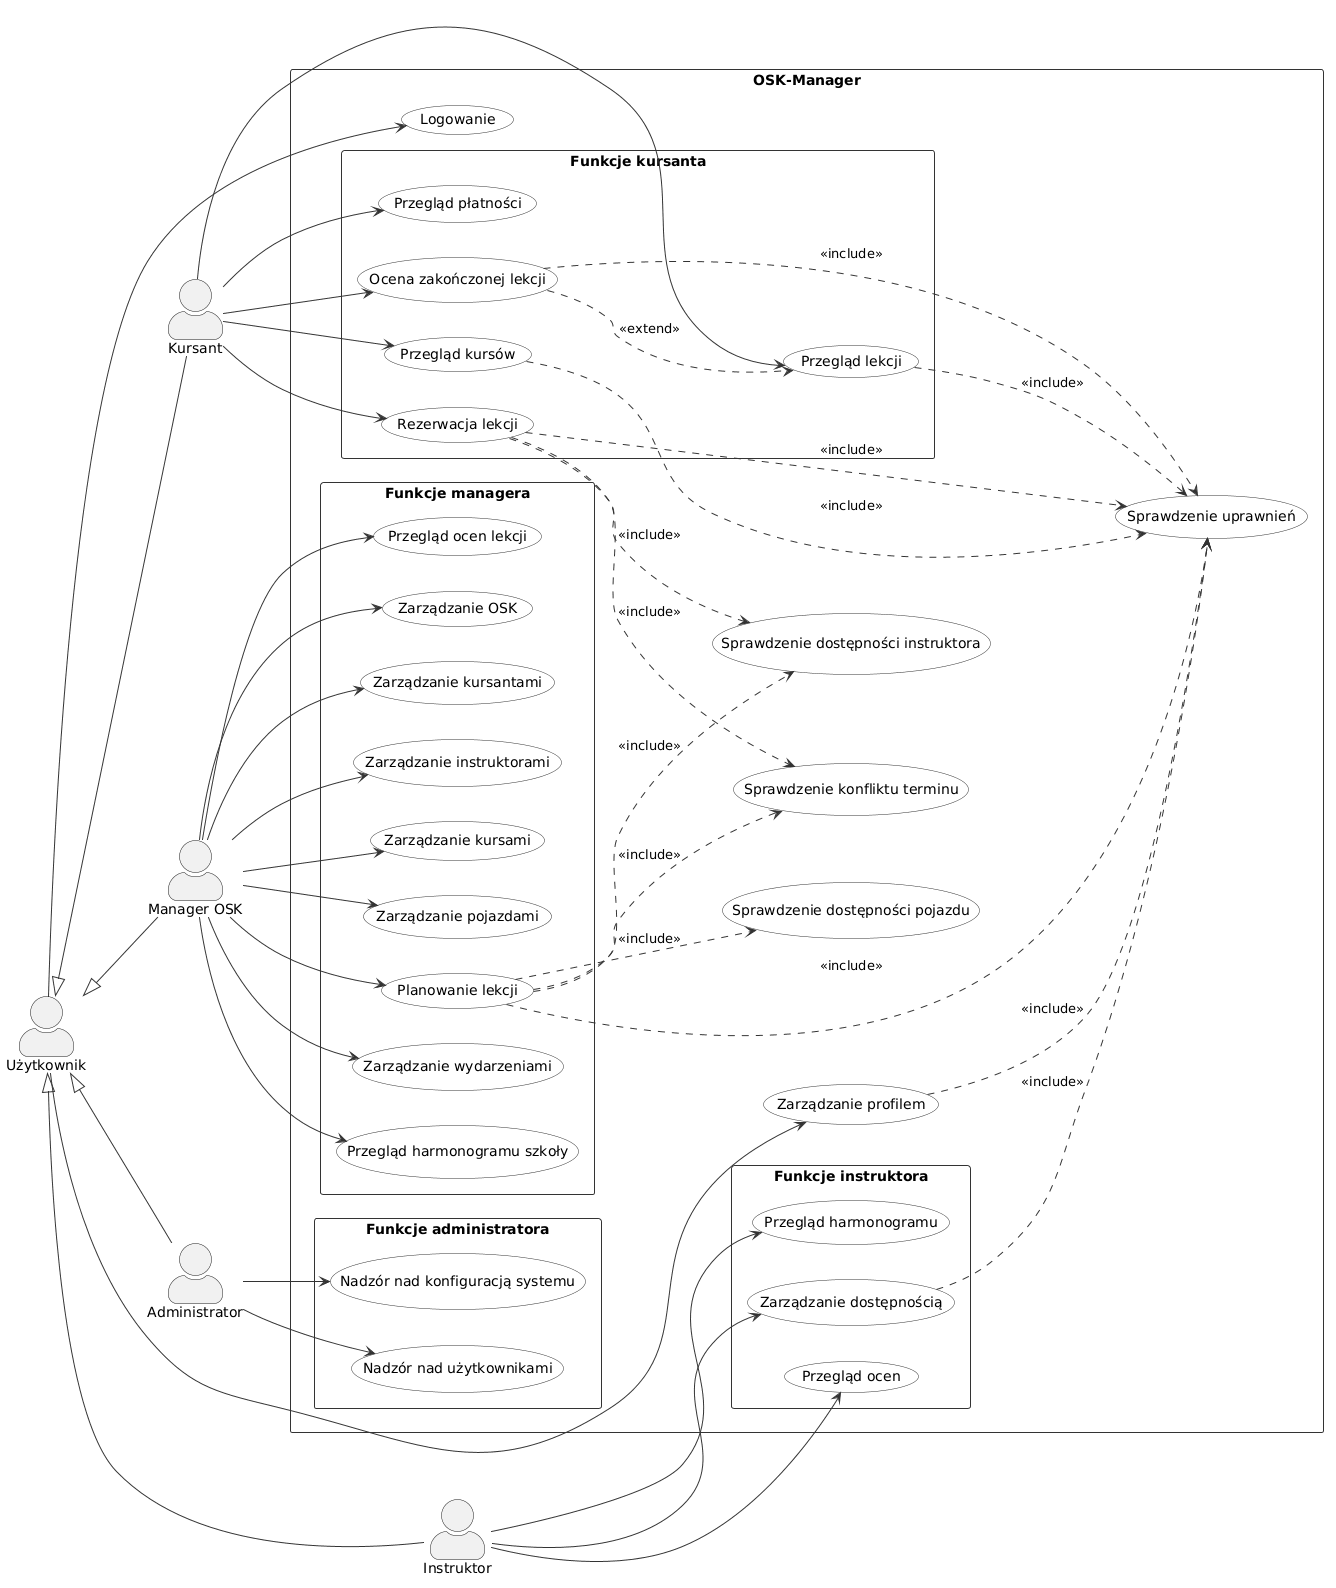
\includegraphics[width=\textwidth,height=0.72\textheight,keepaspectratio]{figures/generated/dpu.png}
\caption{Diagram przypadków użycia systemu OSK-Manager}
\label{fig:dpu-osk-manager}
\wsizsource{Opracowanie własne}
\end{figure}

Przedstawiony diagram celowo pomija szczegóły implementacyjne, takie jak konkretne endpointy API, formularze lub komponenty interfejsu. Takie elementy nie są celem diagramu przypadków użycia. W dokumentacji pełnią one rolę materiału pomocniczego dla dalszych części, przede wszystkim scenariuszy przypadków użycia oraz diagramów aktywności i sekwencji.

\section{Diagram klas}
\label{sec:diagram-klas}

Diagram klas przedstawia uproszczony model domenowy systemu OSK-Manager oraz najważniejsze relacje między obiektami. Model koncentruje się na klasach potrzebnych do opisania głównego procesu biznesowego: zarządzania szkołą jazdy, kursami, lekcjami, instruktorami, pojazdami i płatnościami. Na diagramie celowo pominięto część klas pomocniczych oraz szczegóły techniczne takie jak kontrolery, serwisy, endpointy API i komponenty interfejsu użytkownika.

\begin{figure}[H]
\centering
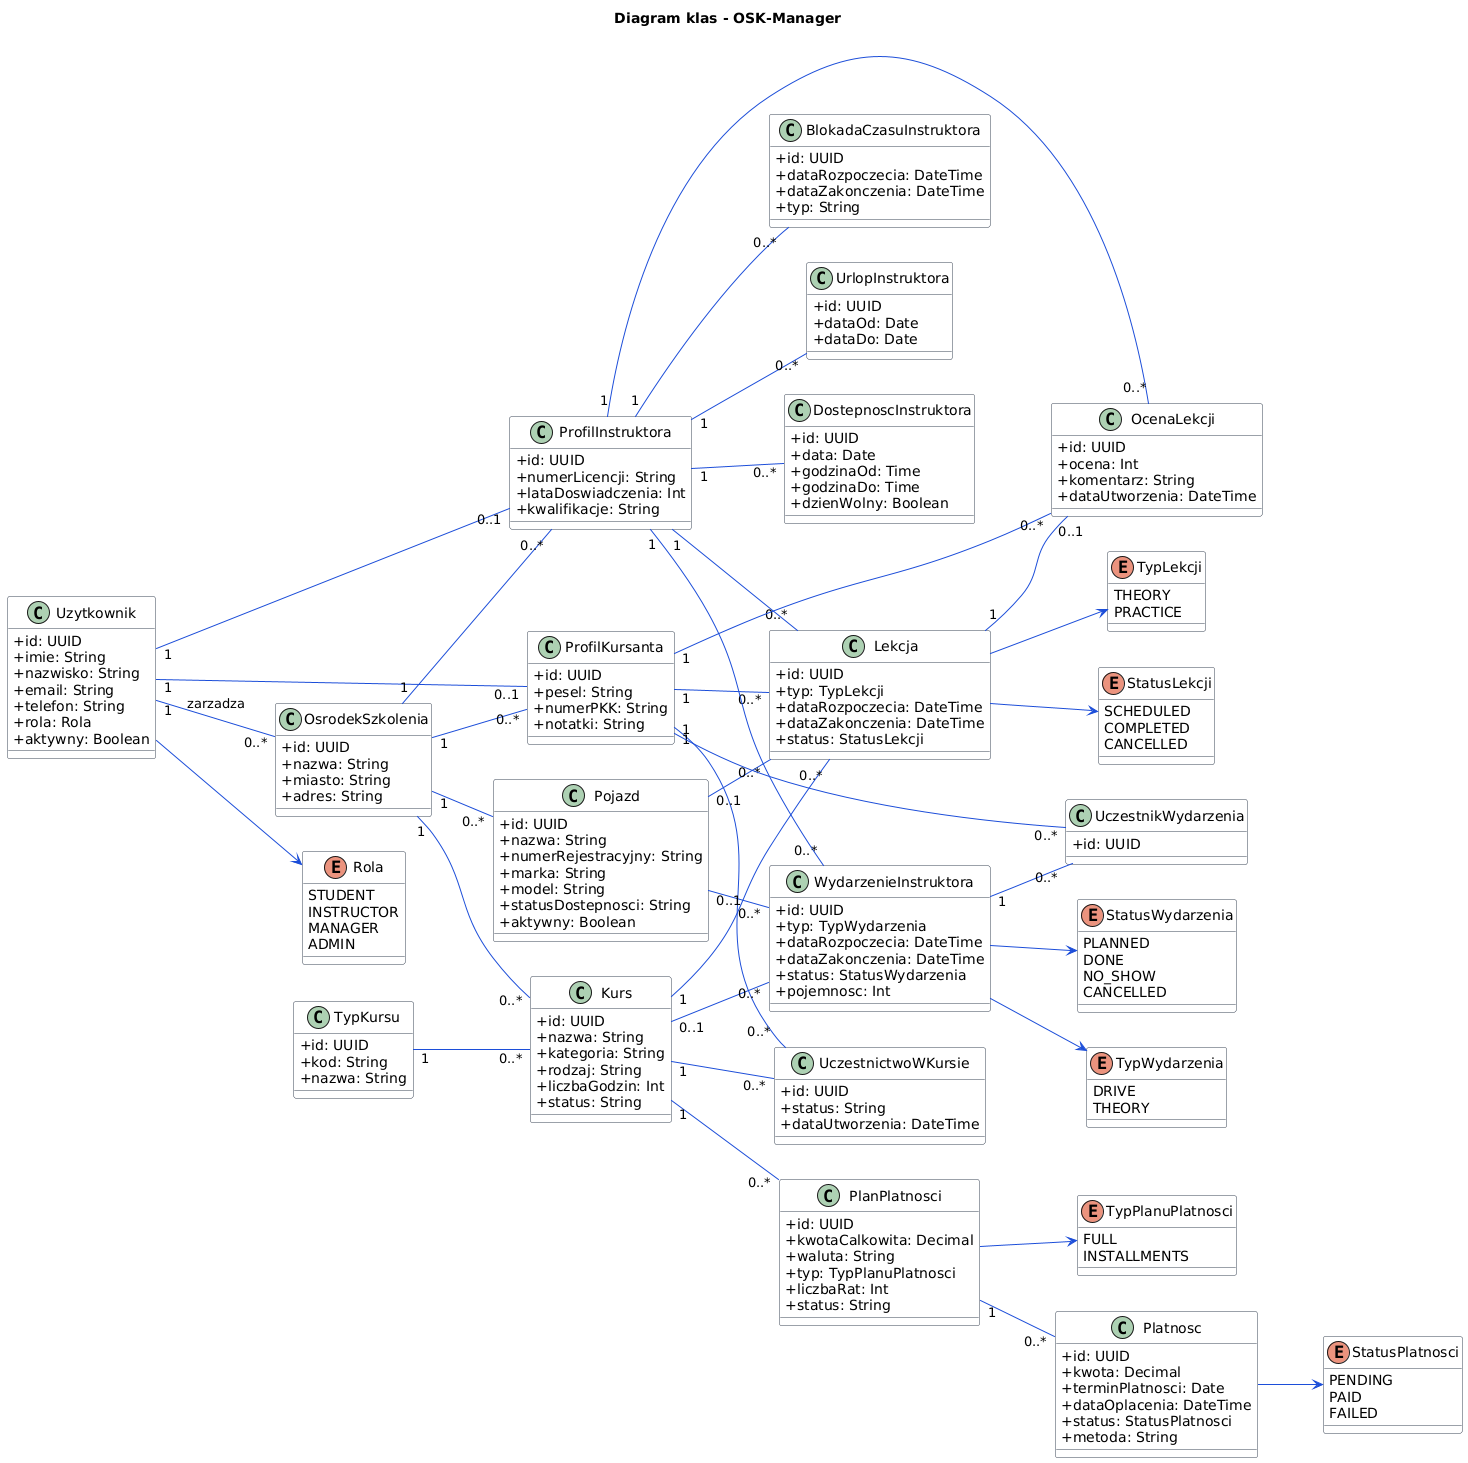
\includegraphics[width=\textwidth,height=0.76\textheight,keepaspectratio]{figures/generated/class-diagram.png}
\caption{Diagram klas systemu OSK-Manager}
\label{fig:diagram-klas-osk-manager}
\wsizsource{Opracowanie własne}
\end{figure}

Klasa \textit{Użytkownik} reprezentuje wszystkie osoby korzystające z systemu, a ich uprawnienia wynikają z przypisanej roli. Ośrodek szkolenia jest centralnym elementem modelu, ponieważ grupuje kursy, pojazdy i użytkowników. Kurs składa się z lekcji, a lekcja praktyczna może być powiązana z pojazdem. Dostępność instruktora wspiera planowanie terminów, natomiast płatności opisują podstawową część rozliczeniową kursu.

\section{Scenariusze przypadków użycia}
\label{sec:scenariusze-przypadkow-uzycia}

Poniżej przedstawiono dwa scenariusze przypadków użycia opisujące kluczowe procesy systemu OSK-Manager. Pierwszy dotyczy pracy managera OSK przy planowaniu lekcji praktycznej, natomiast drugi opisuje działanie kursanta po zakończeniu lekcji.

\subsection{Scenariusz PU-01: Zaplanowanie lekcji praktycznej}
\label{subsec:pu-planowanie-lekcji-praktycznej}

\noindent\textbf{Aktor główny:} Manager OSK.

\noindent\textbf{Cel:} Utworzenie lekcji praktycznej dla kursanta z przypisanym instruktorem, pojazdem oraz terminem.

\noindent\textbf{Warunki początkowe:}
\begin{itemize}
    \item Manager OSK jest zalogowany w systemie.
    \item W systemie istnieje aktywny kursant przypisany do wybranego kursu.
    \item W systemie istnieje instruktor oraz pojazd należący do tego samego ośrodka OSK.
    \item Instruktor ma zdefiniowaną dostępność w harmonogramie.
\end{itemize}

\noindent\textbf{Scenariusz główny:}
\begin{enumerate}
    \item Manager OSK otwiera moduł harmonogramu.
    \item System wyświetla kalendarz zajęć oraz dostępne terminy.
    \item Manager wybiera kursanta i kurs, dla którego ma zostać zaplanowana lekcja.
    \item Manager wybiera typ lekcji jako jazdę praktyczną.
    \item System prezentuje dostępnych instruktorów oraz pojazdy powiązane z danym OSK.
    \item Manager wybiera instruktora, pojazd, datę oraz godzinę rozpoczęcia lekcji.
    \item System sprawdza, czy instruktor i pojazd są dostępni w wybranym terminie.
    \item System sprawdza, czy lekcja należy do właściwego kursu oraz tego samego ośrodka OSK.
    \item Manager zatwierdza utworzenie lekcji.
    \item System zapisuje lekcję i aktualizuje harmonogram.
\end{enumerate}

\noindent\textbf{Scenariusze alternatywne:}
\begin{itemize}
    \item Jeżeli instruktor jest niedostępny, system blokuje zapis i informuje managera o konflikcie terminu.
    \item Jeżeli pojazd jest już przypisany do innej lekcji w tym samym czasie, system blokuje zapis i wymaga wyboru innego pojazdu lub terminu.
    \item Jeżeli wybrany kursant, instruktor lub pojazd nie należy do tego samego OSK, system odrzuca operację.
\end{itemize}

\noindent\textbf{Warunki końcowe:}
\begin{itemize}
    \item Lekcja praktyczna zostaje zapisana w systemie.
    \item Harmonogram kursanta i instruktora zostaje zaktualizowany.
    \item Wybrany pojazd jest oznaczony jako zajęty w czasie trwania lekcji.
\end{itemize}

\subsection{Scenariusz PU-02: Ocena zakończonej lekcji}
\label{subsec:pu-ocena-zakonczonej-lekcji}

\noindent\textbf{Aktor główny:} Kursant.

\noindent\textbf{Cel:} Wystawienie oceny zakończonej lekcji praktycznej.

\noindent\textbf{Warunki początkowe:}
\begin{itemize}
    \item Kursant jest zalogowany w systemie.
    \item Kursant ma przypisaną lekcję praktyczną.
    \item Lekcja ma status zakończony.
    \item Lekcja nie została wcześniej oceniona przez kursanta.
\end{itemize}

\noindent\textbf{Scenariusz główny:}
\begin{enumerate}
    \item Kursant otwiera widok swoich lekcji.
    \item System wyświetla listę lekcji przypisanych do kursanta.
    \item Kursant wybiera zakończoną lekcję praktyczną.
    \item System wyświetla szczegóły lekcji oraz formularz oceny.
    \item Kursant wybiera ocenę i opcjonalnie wpisuje komentarz.
    \item Kursant zatwierdza formularz.
    \item System sprawdza, czy lekcja jest zakończoną lekcją praktyczną i czy nie posiada jeszcze oceny.
    \item System zapisuje ocenę lekcji.
    \item System wyświetla potwierdzenie zapisania oceny.
\end{enumerate}

\noindent\textbf{Scenariusze alternatywne:}
\begin{itemize}
    \item Jeżeli lekcja nie jest zakończona, system nie pozwala wystawić oceny.
    \item Jeżeli lekcja jest lekcją teoretyczną, system nie udostępnia formularza oceny.
    \item Jeżeli lekcja została już oceniona, system pokazuje istniejącą ocenę i blokuje ponowne wystawienie oceny.
    \item Jeżeli kursant próbuje ocenić lekcję innego kursanta, system odmawia dostępu.
\end{itemize}

\noindent\textbf{Warunki końcowe:}
\begin{itemize}
    \item Ocena lekcji zostaje zapisana w systemie.
    \item Kursant może zobaczyć zapisaną ocenę w szczegółach lekcji.
    \item Instruktor i manager OSK mogą wykorzystać ocenę jako informację zwrotną dotyczącą jakości szkolenia.
\end{itemize}

\section{Diagramy aktywności}
\label{sec:diagramy-aktywnosci}

Diagramy aktywności przedstawiają kolejność działań wykonywanych przez użytkowników oraz system w ramach wybranych procesów biznesowych. W dokumentacji systemu OSK-Manager przygotowano dwa diagramy odpowiadające scenariuszom przypadków użycia: zaplanowaniu lekcji praktycznej oraz ocenie zakończonej lekcji.

\subsection{Diagram aktywności: zaplanowanie lekcji praktycznej}
\label{subsec:diagram-aktywnosci-planowanie-lekcji}

Pierwszy diagram przedstawia proces tworzenia lekcji praktycznej przez managera OSK. Szczególną uwagę zwrócono na kontrolę dostępności instruktora i pojazdu, ponieważ są to warunki konieczne do poprawnego zapisania zajęć w harmonogramie.

\begin{figure}[H]
\centering
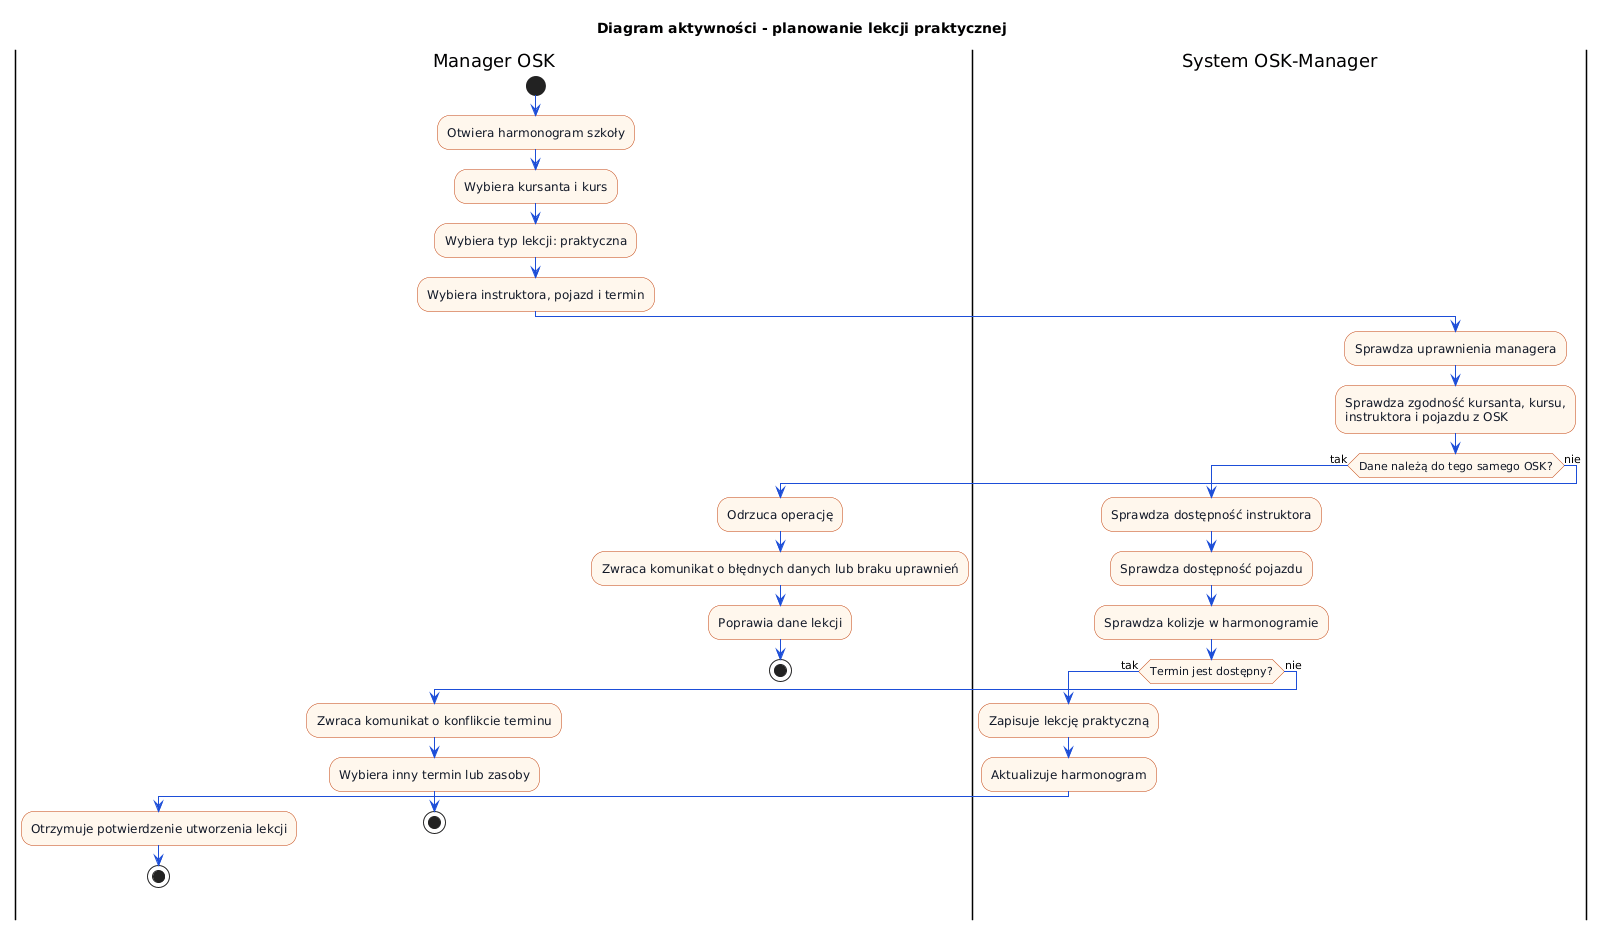
\includegraphics[width=\textwidth,height=0.76\textheight,keepaspectratio]{figures/generated/activity-plan-lesson.png}
\caption{Diagram aktywności procesu planowania lekcji praktycznej}
\label{fig:diagram-aktywnosci-planowanie-lekcji}
\wsizsource{Opracowanie własne}
\end{figure}

\subsection{Diagram aktywności: ocena zakończonej lekcji}
\label{subsec:diagram-aktywnosci-ocena-lekcji}

Drugi diagram przedstawia proces wystawienia oceny lekcji przez kursanta. Proces obejmuje sprawdzenie, czy lekcja została zakończona, czy jest lekcją praktyczną oraz czy nie została wcześniej oceniona.

\begin{figure}[H]
\centering
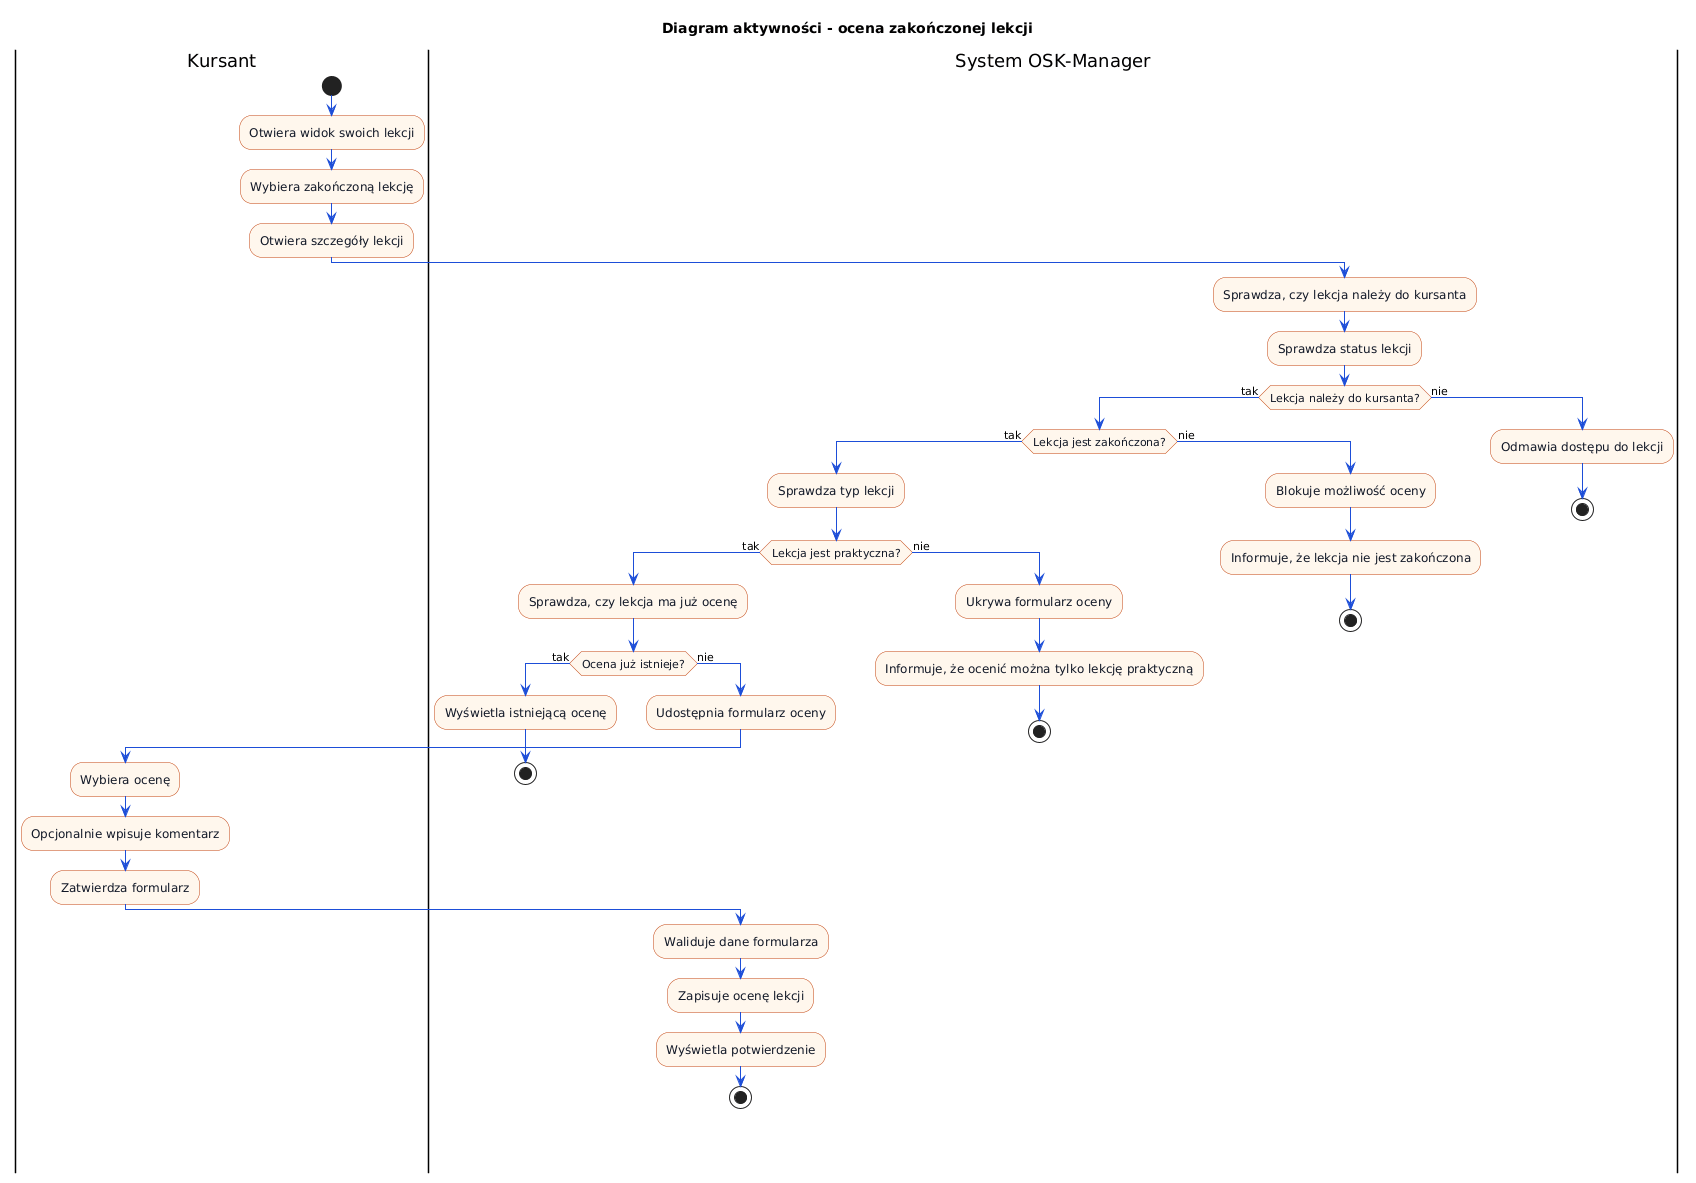
\includegraphics[width=\textwidth,height=0.76\textheight,keepaspectratio]{figures/generated/activity-rate-lesson.png}
\caption{Diagram aktywności procesu oceny zakończonej lekcji}
\label{fig:diagram-aktywnosci-ocena-lekcji}
\wsizsource{Opracowanie własne}
\end{figure}

\section{Diagramy sekwencji}
\label{sec:diagramy-sekwencji}

Diagramy sekwencji przedstawiają wymianę komunikatów pomiędzy uczestnikami procesu w kolejności czasowej. W dokumentacji systemu OSK-Manager przygotowano dwa diagramy odpowiadające kluczowym scenariuszom opisanym wcześniej: zaplanowaniu lekcji praktycznej oraz ocenie zakończonej lekcji. Diagramy pokazują uproszczoną komunikację pomiędzy użytkownikiem, interfejsem aplikacji, backendem oraz bazą danych.

\subsection{Diagram sekwencji: zaplanowanie lekcji praktycznej}
\label{subsec:diagram-sekwencji-planowanie-lekcji}

Pierwszy diagram przedstawia komunikację realizowaną podczas tworzenia lekcji praktycznej przez managera OSK. Szczególnie istotne są zapytania sprawdzające dostępność instruktora i pojazdu, ponieważ od ich wyniku zależy zapis lekcji.

\begin{figure}[H]
\centering
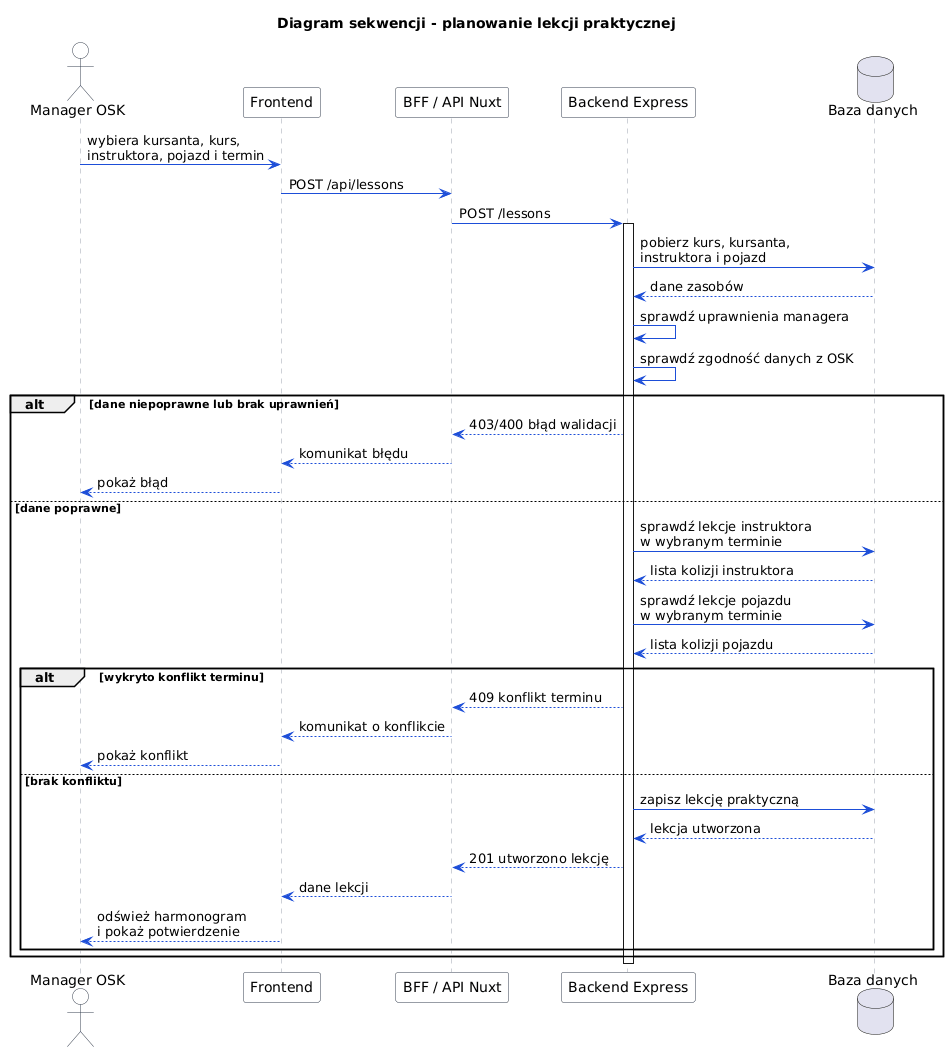
\includegraphics[width=\textwidth,height=0.76\textheight,keepaspectratio]{figures/generated/sequence-plan-lesson.png}
\caption{Diagram sekwencji procesu planowania lekcji praktycznej}
\label{fig:diagram-sekwencji-planowanie-lekcji}
\wsizsource{Opracowanie własne}
\end{figure}

\subsection{Diagram sekwencji: ocena zakończonej lekcji}
\label{subsec:diagram-sekwencji-ocena-lekcji}

Drugi diagram przedstawia komunikację podczas wystawiania oceny zakończonej lekcji przez kursanta. Backend sprawdza, czy lekcja należy do zalogowanego kursanta, czy jest zakończona, czy jest lekcją praktyczną oraz czy nie ma już zapisanej oceny.

\begin{figure}[H]
\centering
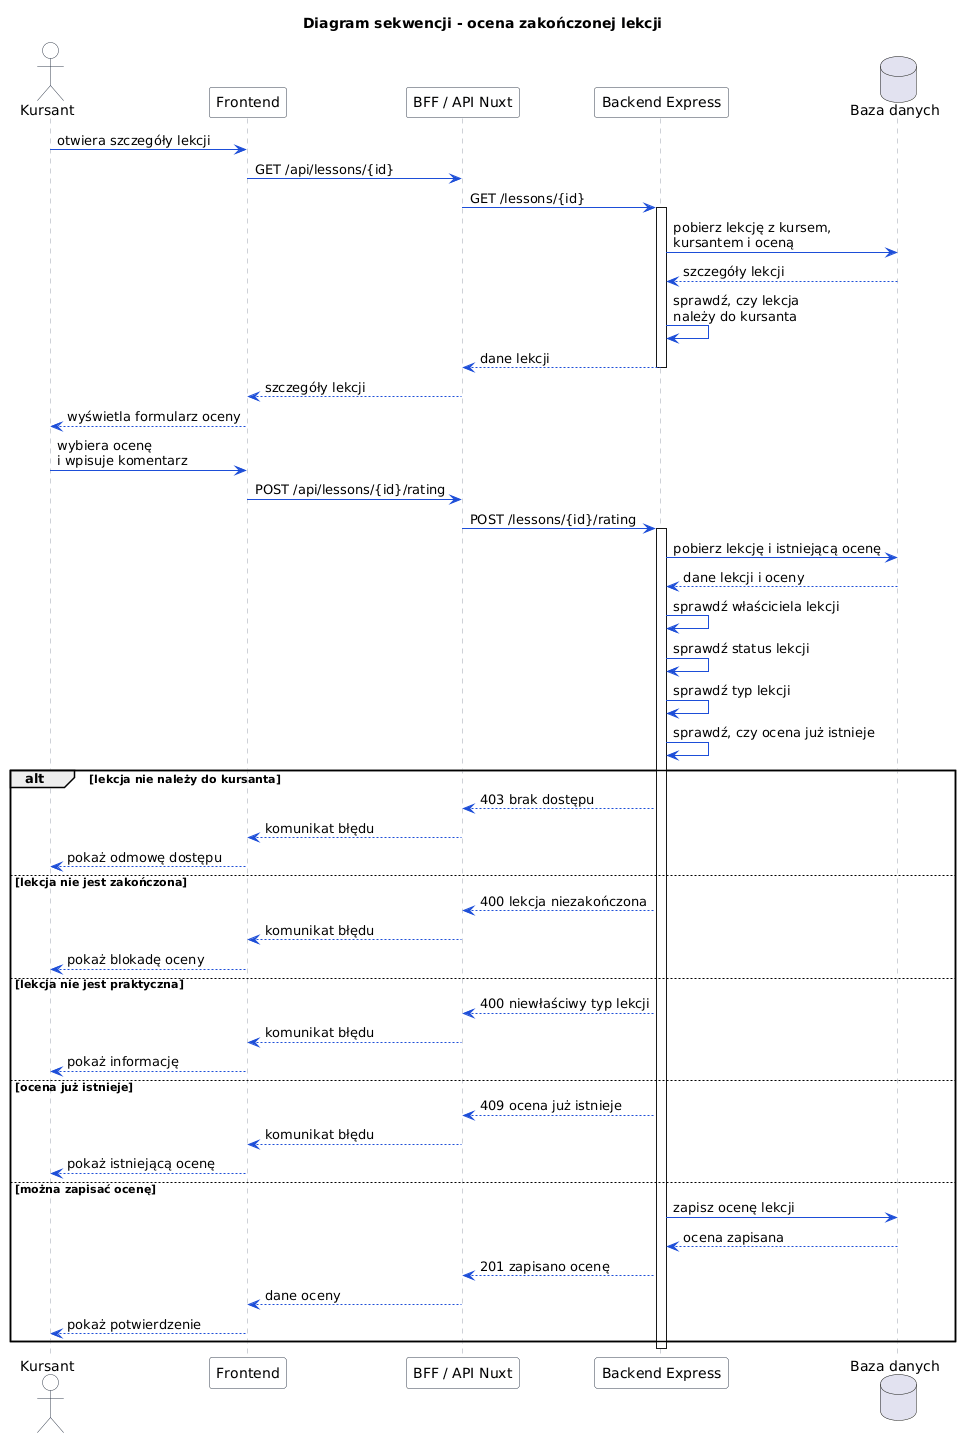
\includegraphics[width=\textwidth,height=0.76\textheight,keepaspectratio]{figures/generated/sequence-rate-lesson.png}
\caption{Diagram sekwencji procesu oceny zakończonej lekcji}
\label{fig:diagram-sekwencji-ocena-lekcji}
\wsizsource{Opracowanie własne}
\end{figure}

\section{Diagramy stanów}
\label{sec:diagramy-stanow}

Diagramy stanów pokazują możliwe stany wybranych obiektów systemu oraz zdarzenia powodujące przejścia pomiędzy nimi. W systemie OSK-Manager szczególnie istotne są cykle życia kursu oraz lekcji, ponieważ wpływają one na harmonogram, dostępność zasobów, panel kursanta oraz rozliczenia.

\subsection{Diagram stanów: kurs}
\label{subsec:diagram-stanow-kurs}

Pierwszy diagram przedstawia uproszczony cykl życia kursu. Kurs po utworzeniu jest przygotowywany organizacyjnie, następnie przechodzi w stan aktywny, a po realizacji wymaganych zajęć może zostać zakończony. W przypadku rezygnacji kursanta lub decyzji managera kurs może zostać anulowany.

\begin{figure}[H]
\centering
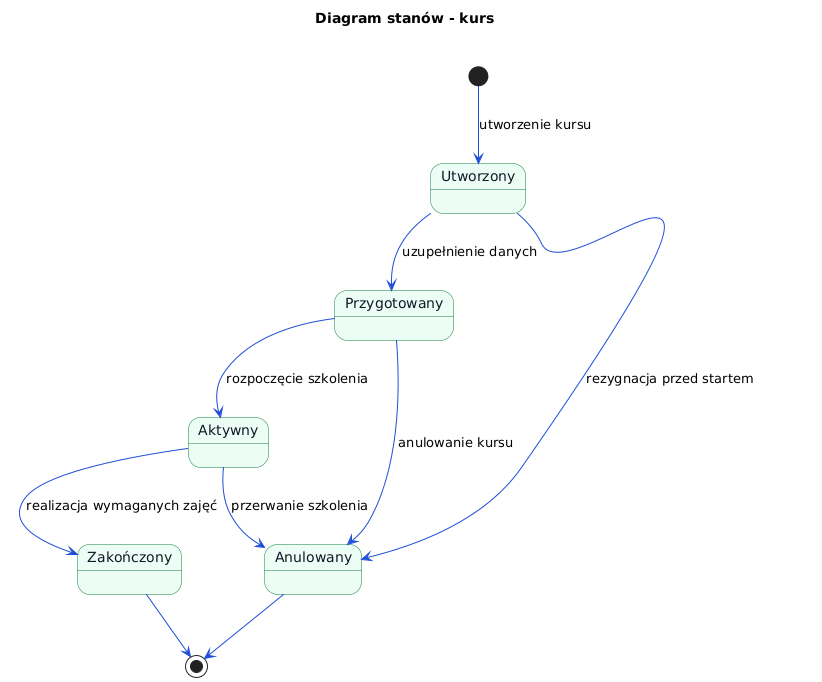
\includegraphics[width=0.78\textwidth,height=0.66\textheight,keepaspectratio]{figures/generated/state-course.png}
\caption{Diagram stanów kursu w systemie OSK-Manager}
\label{fig:diagram-stanow-kurs}
\wsizsource{Opracowanie własne}
\end{figure}

\subsection{Diagram stanów: lekcja}
\label{subsec:diagram-stanow-lekcja}

Drugi diagram przedstawia cykl życia lekcji. Lekcja po zaplanowaniu oczekuje na termin realizacji. Następnie może zostać przeprowadzona i zakończona albo anulowana przed rozpoczęciem. Dla zakończonej lekcji praktycznej możliwe jest zapisanie oceny przez kursanta.

\begin{figure}[H]
\centering
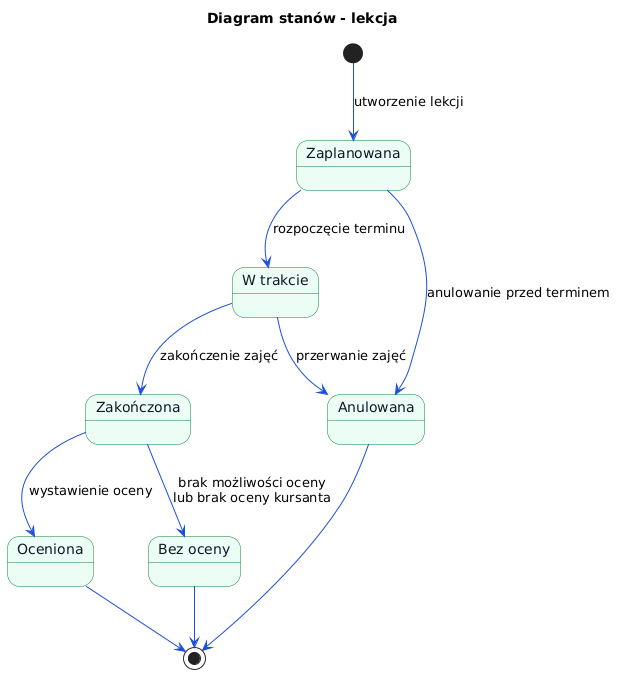
\includegraphics[width=0.78\textwidth,height=0.66\textheight,keepaspectratio]{figures/generated/state-lesson.png}
\caption{Diagram stanów lekcji w systemie OSK-Manager}
\label{fig:diagram-stanow-lekcja}
\wsizsource{Opracowanie własne}
\end{figure}


%------------------------------------------------------------------------------
% Spisy (rysunki / tabele / listingi)
%------------------------------------------------------------------------------
\cleardoublepage
\addcontentsline{toc}{chapter}{Spis rysunków}
\listoffigures

\cleardoublepage
\addcontentsline{toc}{chapter}{Spis tabel}
\listoftables

\cleardoublepage
\addcontentsline{toc}{chapter}{Spis listingów}
\lstlistoflistings

%------------------------------------------------------------------------------
% Bibliografia
%------------------------------------------------------------------------------

\cleardoublepage
\selectlanguage{polish}
\begingroup
  % wyłącz ulem na czas bibliografii
  \renewcommand{\emph}[1]{\textit{#1}}
  \addcontentsline{toc}{chapter}{Bibliografia}
  \bibliographystyle{plain}
  \bibliography{bibliografia}
\endgroup
% przywrócenie ulem (jeśli chcesz)
\renewcommand{\emph}[1]{\uline{#1}}


%------------------------------------------------------------------------------
% Streszczenie PL
%------------------------------------------------------------------------------
\clearpage
\selectlanguage{polish}
\chapter*{}
\label{cha:streszczenie-pl}

\makeatletter

\noindent \textbf{Wyższa Szkoła Informatyki i Zarządzania z siedzibą w Rzeszowie}

\noindent \textbf{Kolegium Informatyki Stosowanej}


\begin{center}
    \textbf{Streszczenie pracy dyplomowej}

    Tytuł pracy w języku polskim 
\end{center}


\noindent \textbf{Autor:}

\noindent \textbf{Promotor:}

\noindent \textbf{Promotor pomocniczy:}

\noindent \textbf{Słowa kluczowe:} (nie więcej niż 200 znaków)

Treść streszczenia, czyli kilka zdań dotyczących treści pracy dyplomowej w języku polskim.



%------------------------------------------------------------------------------
% Streszczenie EN
%------------------------------------------------------------------------------
\clearpage
\selectlanguage{english}
\chapter*{Abstract}
\label{cha:abstract-en}
\makeatletter


\noindent \textbf{The University of Information Technology and Management in Rzeszów}

\noindent \textbf{Faculty of Applied Information Technology}


\begin{center}
    \textbf{Diploma Thesis Summary}

    Tytuł pracy w języku angielskim
\end{center}


\noindent \textbf{Author:}

\noindent \textbf{Supervisor:}

\noindent \textbf{Assistant supervisor:}

\noindent \textbf{Key words:} 

Treść streszczenia, czyli kilka zdań dotyczących treści pracy dyplomowej w języku polskim.





\end{document}
